\documentclass[a4paper]{memoir}
%%%%%%%% CREATE DOCUMENT STRUCTURE %%%%%%%%
\usepackage[utf8]{inputenc}
\usepackage[english]{babel}
\usepackage{pdfpages}
\usepackage[T1]{fontenc}
\usepackage{appendix}
\usepackage[a4paper,top=2.2cm,bottom=2.2cm,left=2.2cm,right=2.2cm,marginparwidth=1.75cm]{geometry}
\usepackage{graphicx}
\usepackage[figuresleft]{rotating}
\usepackage{siunitx}
\usepackage{booktabs}
\usepackage{longtable}
\usepackage{csquotes}
\usepackage{textcomp}
\usepackage{gensymb}
\usepackage{amsmath}
\usepackage{comment}
\usepackage{graphicx}
\usepackage{wasysym}
\usepackage{subcaption}
\usepackage{titlesec}
\usepackage{listings}
\usepackage{appendix}
\usepackage[colorinlistoftodos]{todonotes}
\usepackage[colorlinks=true, allcolors=black]{hyperref}
\addto\extrasenglish{
    \def\chapterautorefname{Chapter}
    \def\sectionautorefname{Section}
    \def\subsectionautorefname{Subsection}
    \def\subsubsectionautorefname{Subsubsection}
}
\usepackage{listings}
\usepackage{xcolor} % for custom colours
\lstset{
    language=Python,
    basicstyle=\ttfamily\small,
    commentstyle=\color{green},
    keywordstyle=\color{blue},
    stringstyle=\color{red},
    showstringspaces=false,
    numbers=left,
    numberstyle=\tiny,
    numbersep=10pt,
    breaklines=true,
    frame=single,
    captionpos=b
}

\usepackage{caption}
\usepackage{multicol}
\usepackage{float}
\usepackage[official]{eurosym}
\usepackage{adjustbox}
\usepackage{titling} 
\usepackage{blindtext}
\usepackage{atbegshi}
\usepackage{tikz}
\usepackage{pdfpages}
\usepackage{wrapfig}
\usepackage{listings}
\usepackage{xcolor}
\usepackage{subcaption}
\let\Square\relax
\usepackage{bbding}
\usepackage{tocvsec2}
\usepackage{siunitx}
\usepackage{amsmath}
\usepackage{authblk}
\usepackage{caption}
\definecolor{codegreen}{rgb}{0,0.6,0}
\definecolor{codegray}{rgb}{0.5,0.5,0.5}
\definecolor{codepurple}{rgb}{0.58,0,0.82}
\definecolor{backcolour}{rgb}{0.95,0.95,0.92}
\definecolor{deepskyblue}{rgb}{0.0, 0.75, 1.0}

\lstdefinestyle{mystyle}{
    backgroundcolor=\color{backcolour},   
    commentstyle=\color{codegreen},
    keywordstyle=\color{magenta},
    numberstyle=\tiny\color{deepskyblue},
    stringstyle=\color{codepurple},
    basicstyle=\ttfamily\footnotesize,
    breakatwhitespace=false,         
    breaklines=true,                 
    captionpos=b,                    
    keepspaces=true,                 
    numbers=left,                    
    numbersep=5pt,                  
    showspaces=false,                
    showstringspaces=false,
    showtabs=false,                  
    tabsize=2
}

\lstset{style=mystyle}

\usepackage[style=ieee, citestyle=numeric]{biblatex}
\addbibresource{Bibliography.bib}
\DeclareFieldFormat{labelnumberwidth}{\mkbibbrackets{#1}}
\defbibenvironment{bibliography}
  {\list
     {\printtext[labelnumberwidth]{
      \printfield{labelprefix}
      \printfield{labelnumber}}}
     {\setlength{\labelwidth}{\labelnumberwidth}
      \setlength{\leftmargin}{\labelwidth}
      \setlength{\labelsep}{\biblabelsep}
      \addtolength{\leftmargin}{\labelsep}
      \setlength{\itemsep}{\bibitemsep}
      \setlength{\parsep}{\bibparsep}}
      \renewcommand*{\makelabel}[1]{\hss##1}}
  {\endlist}
  {\item}
\definecolor{darkgreen}{rgb}{0.0, 0.4, 0.0}
\usepackage{xcolor,fix-cm}
\definecolor{numbercolor}{rgb}{0.0, 0.75, 1.0}
\newif\ifchapternonum
\makechapterstyle{jenor}{
\setlength{\beforechapskip}{0cm}
\setlength{\afterchapskip}{0.5cm}
\renewcommand\printchaptername{}
\renewcommand\printchapternum{}
\renewcommand\printchapternonum{\chapternonumtrue}
\renewcommand\chaptitlefont{\fontfamily{cmr}\fontseries{db}
\fontshape{n}\fontsize{25}{35}\selectfont\raggedleft}
\renewcommand\chapnumfont{\fontfamily{pbk}\fontseries{m}\fontshape{n}
\fontsize{0.7in}{0in}\selectfont\color{numbercolor}}
\renewcommand\printchaptertitle[1]{
\noindent
\ifchapternonum
\begin{tabularx}{\textwidth}{X}
{\parbox[t]{\linewidth}{\chaptitlefont ##1}
\vphantom{\raisebox{-7pt}{\chapnumfont 1}}}
\end{tabularx}
\else
\begin{tabularx}{\textwidth}{Xl}
{\parbox[t]{\linewidth}{\chaptitlefont ##1}}
& \raisebox{-7pt}{\chapnumfont \thechapter}
\end{tabularx}
\fi
\par\vskip1mm\hrule}}
\chapterstyle{jenor}

\renewcommand\cftappendixname{\appendixname~}
\setlength{\marginparwidth}{2.2cm}
\openany

\settocdepth{section}
\setsecnumdepth{subsection}


\begin{document}
\setlength{\parindent}{0em}

\AtBeginShipoutNext{\AtBeginShipoutNext{\AtBeginShipoutDiscard}}
\begin{titlingpage}

\mainmatter 

\newcommand{\HRule}{\rule{\linewidth}{0.5mm}} 				
\center 
\textsc{\Large Delft University of Technology}\\[0.5cm]
\textsc{\Large Faculty of Aerospace Engineering}\\[0.2cm]
% \textsc{\Large AE3212-II}\\[0.2cm]
\textsc{\large 
Rotor / wake Aerodynamics - AE4135 }\\[1cm] 							
\HRule \\[0.5cm]
{ \huge \bfseries 
Rotor / wake Aerodynamics \\ \large{\emph{Assignment 1: Blade Element Theory}} }\\[0.2cm]
%{ \Large }\\[0.2cm]
\HRule \\[0.5cm]
\large
Instructor: Prof. Dr.ir. C.J. Simao Ferreira \\
Julian Gonzalez, 6281486 \\
Stijn Hersbach, 4857054 \\
Pim Haanen, 5092795 \\
\large{\large \today}\\
\vspace{5pt}
\HRule \\[0.5cm]
\vspace{5pt}





\begin{figure}[b]
\centering

\includegraphics[width=0.15\textwidth]{Figures/tu_delft_logo_jpg.png}
\end{figure}
\end{titlingpage}
\pagestyle{ruled}

\large
% \frontmatter

% \input{Chapters/Summary}
% \newpage

\begin{KeepFromToc}
    \tableofcontents
\end{KeepFromToc}

% \newpage
% \listoftables
% \newpage
% \listoffigures
% \newpage
% \input{Chapters/Lists}
% \newpage
\setcounter{page}{2}

\chapter{Nomenlacture}
\begin{align*}
\alpha & \quad \text{angle of attack at blade element} \, (-) \\
\beta & \quad \text{blade twist angle at blade element} \, (-) \\
\lambda & \quad \text{tip speed ratio} \, (-) \\
\rho & \quad \text{fluid density} \, (\text{kg} \cdot \text{m}^{-3}) \\
\Gamma & \quad \text{circulation at blade element} \, (\text{m}^2 \cdot \text{s}^{-1}) \\
\Phi & \quad \text{perceived-wind inflow-angle at blade element} \, (-) \\
\Omega & \quad \text{rotor rotational velocity} \, (\text{rad} \cdot \text{s}^{-1}) \\
a & \quad \text{axial induction factor} \, (-) \\
a' & \quad \text{azimuthal induction factor} \, (-) \\
c & \quad \text{blade element chord} \, (\text{m}) \\
C_d & \quad \text{drag coefficient} \, (-) \\
C_l & \quad \text{lift coefficient} \, (-) \\
C_T & \quad \text{thrust coefficient} \, (-) \\
\text{Drag} & \quad \text{drag force per unit span} \, (\text{N} \cdot \text{m}^{-1}) \\
\text{Lift} & \quad \text{lift force per unit span} \, (\text{N} \cdot \text{m}^{-1}) \\
F_{\text{azim}} & \quad \text{azimuthal/tangential force per unit span} \, (\text{N} \cdot \text{m}^{-1}) \\
F_{\text{axial}} & \quad \text{axial force per unit span} \, (\text{N} \cdot \text{m}^{-1}) \\
N_{\text{blades}} & \quad \text{number of blades} \, (-) \\
V_{\text{axial}}=U_{\text{rotor}} & \quad  \text{ axial velocity perceived by blade element, axial velocity at rotor} \, (\text{m} \cdot \text{s}^{-1}) \\
V_P & \quad \text{velocity perceived by blade element} \, (\text{m} \cdot \text{s}^{-1}) \\
V_{\text{tan}} & \quad \text{azimuthal/tangential velocity perceived by blade element} \, (\text{m} \cdot \text{s}^{-1})
\end{align*}

\chapter{Introduction} \label{ch:Introduction}

% Please add the following required packages to your document preamble:
% \usepackage{longtable}
% Note: It may be necessary to compile the document several times to get a multi-page table to line up properly
\begin{longtable}{|l|r|}
\caption{Wind turbine geometrical specifications}
\label{tab:turbinegeometry}\\
\hline
\multicolumn{1}{|c|}{\textbf{Variable}} & \multicolumn{1}{c|}{\textbf{Value}} \\ \hline
\endhead
%
Radius (R)                              & 50 {[}m{]}                          \\ \hline
Number of Blades                        & 3                                   \\ \hline
Blade starts at                         & 0.2 r/R                             \\ \hline
Twist                                   & 14*(1-r/R) {[}degrees{]}            \\ \hline
Blade Pitch                             & -2 {[}degrees{]}                    \\ \hline
Chord Distribution                      & 3*(1-r/R)+1 {[}m{]}                 \\ \hline
Airfoil                                 & DU 95-W-180                         \\ \hline
Rotor yaw angle                         & 0, 15 and 30 {[}degrees{]}          \\ \hline
\end{longtable}

% Please add the following required packages to your document preamble:
% \usepackage{longtable}
% Note: It may be necessary to compile the document several times to get a multi-page table to line up properly
\begin{longtable}{|l|l|}
\caption{Wind turbine operational specifications}
\label{tab:operspecs}\\
\hline
\textbf{Variable}        & \textbf{Value}          \\ \hline
\endhead
%
Wind speed (U0)          & 10 {[}m/s{]}            \\ \hline
Tip speed ratio ($\lambda$) & 6, 8, 10                \\ \hline
Rotor yaw angle          & 0, 15, 30 {[}degrees{]} \\ \hline
\end{longtable}

\begin{figure}
    \centering
    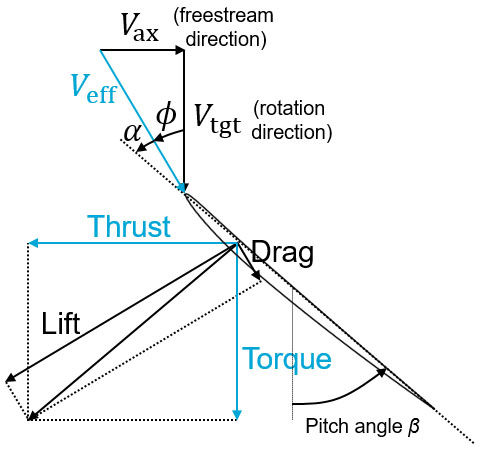
\includegraphics[width=0.5\textwidth]{Figures/velocitydiagram.jpg}
    \caption{Caption}
    \label{fig:enter-label}
\end{figure}
\chapter{Flow diagram of the code}

\begin{figure}[H]
    \centering
    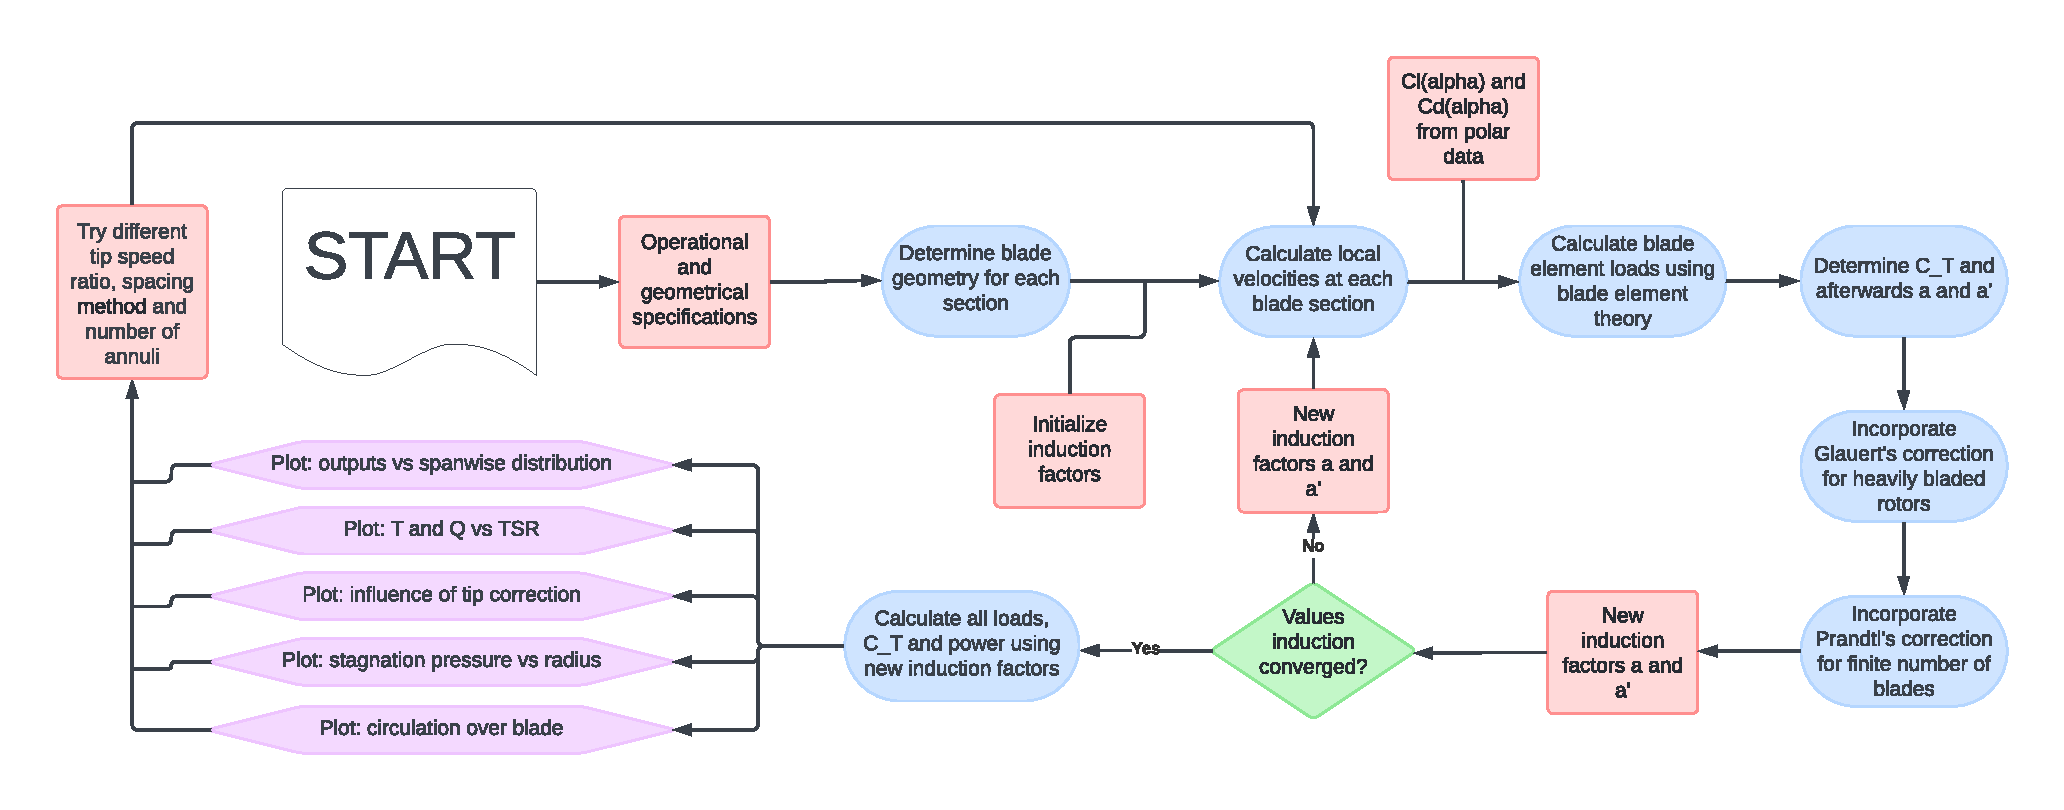
\includegraphics[width=\textwidth]{Figures/Blank diagram.pdf}
    \caption{Flow diagram of the code}
    \label{fig:enter-label}
\end{figure}

\section{Assumptions}
\begin{itemize}
    \item \textbf{Steady Flow:} the flow characteristics are assumed to be independent of time.
    \item \textbf{Inviscid Flow:} the flow is assumed to be inviscid. This means no viscous effects are taken into account.
    \item \textbf{Incompressible Flow:} the flow is assumed to be incompressible. This means the density throughout the streamtube is constant. This enables the use of Bernoulli's equation in locations of a continuous pressure distribution. This also results in the product of area and flow velocity being constant over the flow.
    \item \textbf{2D Flow:} it is assumed that the flow characteristics can accurately be modeled using 2 dimensional flow characteristics.
    \item \textbf{Constant Internal Energy:}  it is assumed that the internal energy within the streamtube is constant so there no radiation, convection or conduction occurring.
    \item \textbf{Independent annulus:} the annuli are considered independently of one another. In reality, flow characteristics on one annulus will influence the characteristics on another (cross flow), this effect is ignored.
    \item \textbf{Circular Discs:} the actuator disc in the model is assumed to be of circular shape. In reality slight changes in the shape could occur, these are neglected.
    \item \textbf{Root-section:} it is assumed that the root section till $r/R = 0.2$ has no influence on the performance of the turbine and can be neglected.
\end{itemize}
\chapter{Results}

\section{Reference Data (for cl(alpha) and cd(alpha))}
\begin{figure}
    \centering
    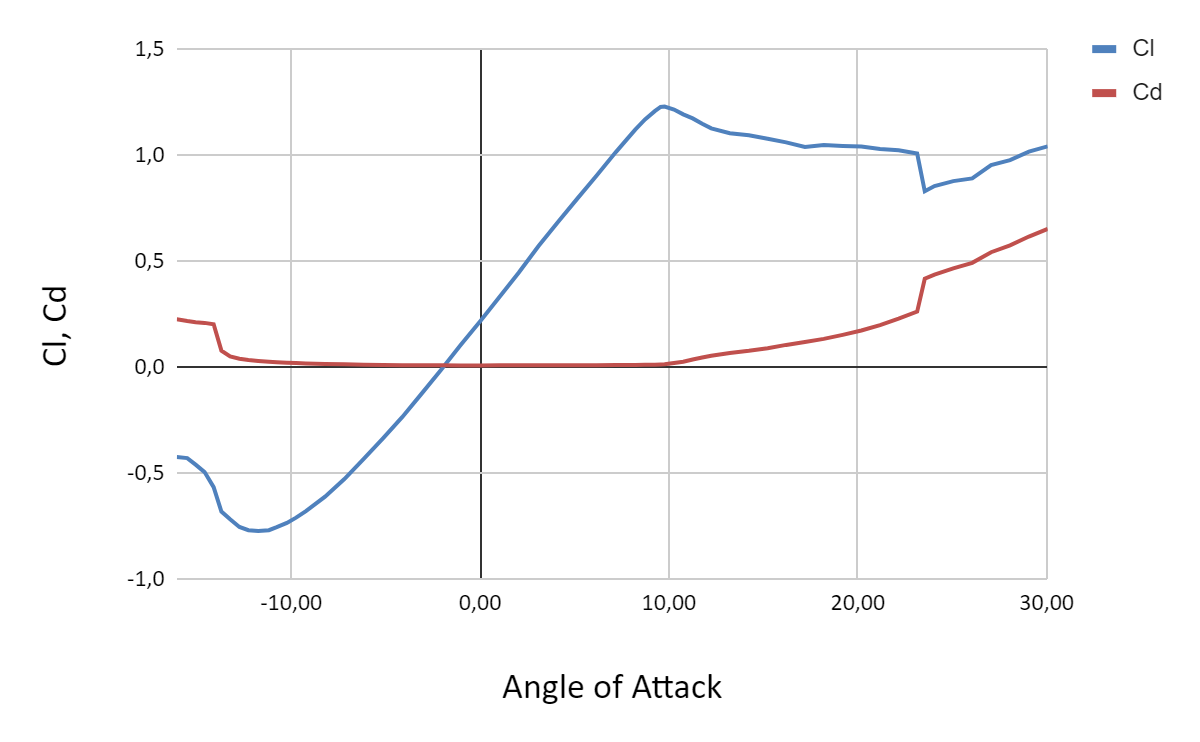
\includegraphics[width=0.5\textwidth]{Figures/REF_CLCDALPHA.png}
    \caption{Caption}
    \label{fig:enter-label}
\end{figure}
\begin{figure}
    \centering
    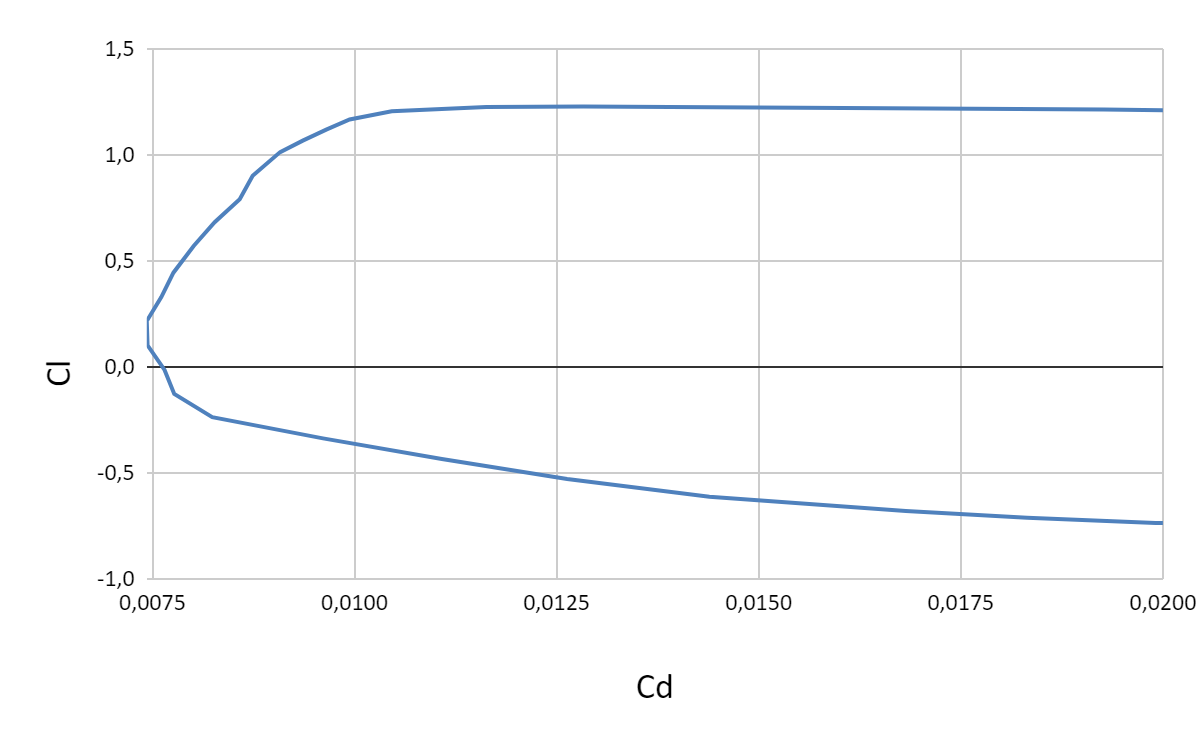
\includegraphics[width=0.5\textwidth]{Figures/REF_CLCD.png}
    \caption{Caption}
    \label{fig:enter-label}
\end{figure}
\begin{figure}
    \centering
    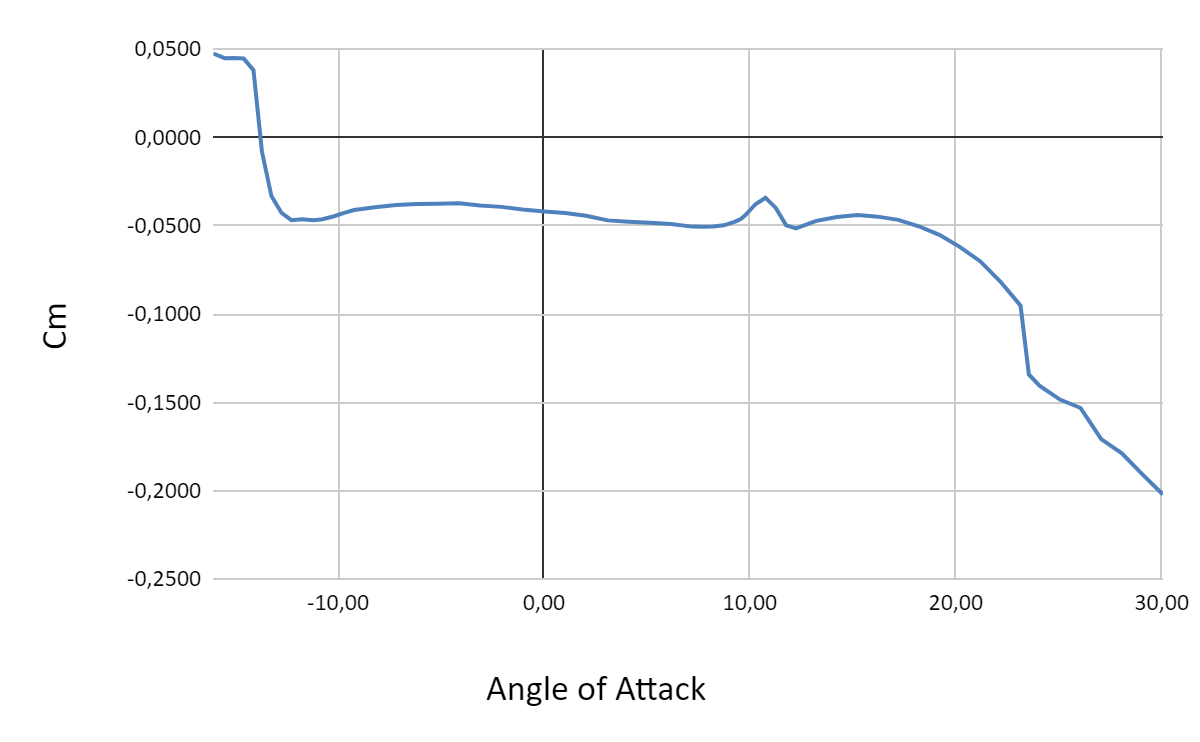
\includegraphics[width=0.5\textwidth]{Figures/REF_CMALPHA.png}
    \caption{Caption}
    \label{fig:enter-label}
\end{figure}
\chapter{Conclusion}
\chapter{Python Script}


\printbibliography[heading=bibintoc,title=References]


\end{document}

